\item \points{4c}
\textbf{Duble descent phenomenon and the effect of regularization. }

In this question, we will show that regularization mitigates the double descent phenomenon for linear regression. We will use the same datasets as specified in sub-question (b). Now consider using various regularization strengths. For $\lambda\in \{0, 1, 5, 10, 50, 250, 500, 1000\}$, you will compute the minimizer of $J_\lambda(\beta).$ 

Complete the \texttt{ridge\_regression} method of \texttt{src-doubledescent/submission.py} which takes in a training file and a validation file, computes the $\hat{\beta}_\lambda$ that minimizes the training objective under different regularization strengths, and returns a list of validation errors (one for each choice of $\lambda$).



The output plot should look similar to the following (no plot submission is required):

\begin{figure}[H]
    \centering
    \vspace{-2mm}
    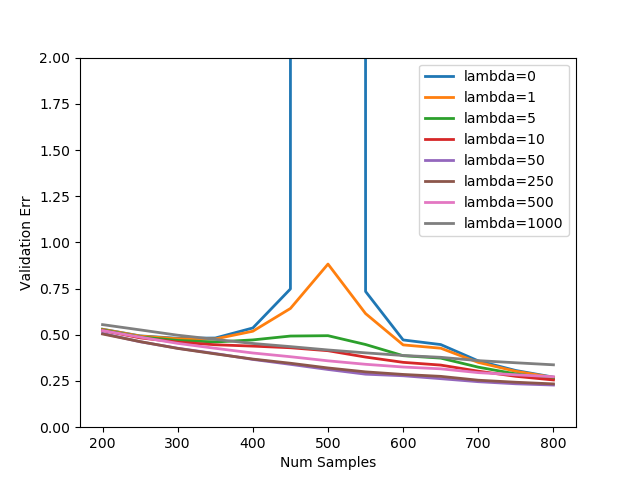
\includegraphics[width=0.65\linewidth]{04-doubledescent/reg.png}
    \caption{Num of samples vs. validation error for different regularization strengths}
    \centering
\end{figure}


The x-axis is the size of the training dataset (from 200 to 800); the y-axis is the MSE on the validation dataset.


You should observe that for some small $\lambda$'s, the validation error may increase and then decrease as we increase the sample size. However, double descent does not occur for a relatively large $\lambda$. 


\textbf{Remark:} If you want to learn more about the double descent phenomenon and the effect of regularization, you can start with this paper \href{https://arxiv.org/abs/2003.01897}{Nakkiran, et al. 2020}.